\documentclass{hipatia}
\usepackage{graphicx}
%\graphicspath{efemerides/}
\title{Eventos DMAT \\ Janeiro a Dezembro/25}
\subtitle{Simpósio}
\author{Cristina Lizana, Elaís Cidely Malheiro, Henrique da Costa, Roberto Sant'Anna}


%\makeindex
\newcommand{\superau}{\textsuperscript{\underline{a}}~}
\newcommand{\superou}{\textsuperscript{\underline{o}}~}
%\newcommand{\sepdecorada}{%
%  \vspace{0.4cm} % Espaço antes
%  \begin{center}
%    \begin{tikzpicture}
%     % Cria uma linha de 5 ornamentos (índices -2, -1, 0, 1, 2)
%      \foreach \x in {-2,-1,0,1,2}
%        \node[color=olivadark] at (\x*1.1,0) {\pgfornament[width=1.1cm]{39}};
%    \end{tikzpicture}
%  \end{center}
%  \vspace{0.1cm} % Espaço depois (curto para colar no título)
%}
\titleformat{\section}{\color{cinza}\normalfont\large\bfseries}{}{0em}{}
\begin{document}
\setcounter{page}{\simposiopage}
\maketitle

%\printindex

%\tableofcontents
%\addcontentsline
%\addtocontents

%\section{Introdução}

Nesta seção \textsc{Simpósio}  faremos uma breve resenha de eventos organizados por membros da comunidade do Departamento de Matemática (DMAT) do Instituto de Matemática e Estatística (IME) da Universidade Federal da Bahia (UFBA) durante o período de janeiro a dezembro de 2025. 

%\vspace{0.5cm}

\sepdecorada

%\begin{center}
\noindent {\Large\textbf{\textsc{Cenário Científico e Pós-Graduação}}}
%\end{center}

\noindent \textit{Iniciamos nossa retrospectiva destacando os eventos que conectaram o DMAT à fronteira do conhecimento, reunindo pesquisadores de diversas partes do mundo e fortalecendo a pós-graduação e a produção científica.}


%%%% BLOCO 1 %%%%

\section{Formação de Professores de Matemática no Verão da UFBA}

Realizado no dia 31 de janeiro de 2025, no Auditório do IME-UFBA, o evento ``Formação de Professores de Matemática no Verão da UFBA'' teve como um dos principais objetivos contribuir para a melhoria do ensino de Matemática na Educação Básica. Diante dos desafios apontados por índices nacionais, a atividade ofereceu um conjunto de palestras voltadas ao desenvolvimento de saberes práticos e estratégias pedagógicas inovadoras.

A organização foi uma parceria entre o Programa de Iniciação à Docência (PIBID-UFBA/Matemática) e o Mestrado Profissional em Matemática em Rede Nacional (PROFMAT-UFBA), sob a coordenação das professoras Graça Dominguez e Elaís Cidely.

A programação científica destacou-se pela abordagem de temas contemporâneos. O professor Rogério Steffenon (UNISINOS) proferiu a palestra ``Belos Problemas de Matemática'', explorando o raciocínio lógico e o reconhecimento de padrões.

\begin{figure}[htb]
    \centering
    \includegraphics[width=8.5cm]{verao_rogerio.jpg}
    \caption{Prof.\ \  Rogério Steffenon (UNISINOS) durante sua apresentação sobre problemas matemáticos.}
    \label{fig:verao_rogerio}
\end{figure}


Em seguida, o professor Luciano Guimarães (FGV) discutiu ``Problemas de Olimpíada na sala de aula'', apresentando técnicas estratégicas para o ambiente escolar. Encerrando o ciclo, o professor Krerley Oliveira (UFAL) apresentou o ``NES - Novo Ensino Suplementar'', uma proposta inovadora para o Ensino Médio que integra Ciência de Dados e Inteligência Artificial.

\begin{figure}[htb]
    \centering
    \includegraphics[width=8.5cm]{verao_luciano.jpg}
    \caption{Prof.\ \  Luciano Guimarães (FGV) discutindo o uso de problemas olímpicos em sala de aula.}
    \label{fig:verao_luciano}
\end{figure}

As atividades demonstraram uma sólida articulação entre teoria e prática, vinculando-se tanto às disciplinas das Licenciaturas quanto às pesquisas do PROFMAT. Com um público de aproximadamente 70 participantes, o encontro foi marcado por trocas de experiências que incentivam o uso de abordagens criativas no contexto escolar.

\begin{figure}[htb]
    \centering
    \includegraphics[width=8.5cm]{verao_plateia.jpg}
    \caption{Público presente no Auditório do IME durante o evento de formação.}
    \label{fig:verao_plateia}
\end{figure}

\section{XVIII ENAMA}

O Encontro Nacional de Análise Matemática e Aplicações (ENAMA) teve sua 18\textsuperscript{\underline{a}} edição sediada no IME - UFBA entre os dias 2 e 5 de novembro de 2025. O tradicional evento anual, que ocorre desde 2005, reúne professores e pesquisadores de todas as regiões do Brasil e também do exterior, e tem o propósito de criar debates nas áreas de Análise Funcional, Análise Numérica, Equações Diferenciais Parciais, Ordinárias e Funcionais.

Na edição deste ano foram mais de 100 inscritos e 80 trabalhos apresentados, entre eles os convidados Alexandre Nolasco Carvalho (ICMC - USP), Enrique Zuazua (\textit{Friedrich-Alexander-Universität}, Alemanha), Fernando Costa Jr (UFPB), Jaqueline Godoy Mesquita (Unicamp) e Sandra Moreira Neto (UEMA).

\begin{figure}[htb]
    \centering
    \includegraphics[width=7.5cm]{Enama-mesa.jpg}
    \caption{Mesa de abertura do XVIII ENAMA.}
 \label{fig:enama_abertura}
\end{figure}

O encontro é reconhecido por unir novos e renomados pesquisadores e ter espaço convidativo para que todos participem, fato que influencia positivamente a carreira dos participantes, muitos dos quais sempre retornam ao evento. Entre as diversas palestras e minicursos apresentados ocorreram também atividades sociais, incluindo um jantar oficial e culinária típica.

Tanto a organização local, encabeçada por Arthur Cunha (UFBA) e composta por Henrique Costa (UFBA), Juan González (UFBA), Roseane Martins (UESC), Carlos Raposo (UFPA), Joilson Ribeiro (UFBA) e Leandro Araújo (UESB), quanto o comitê nacional, composto por Haroldo Clark (UFDPar), Joedson Santos (UFPB) e Sandra Malta (LNCC), foram elogiados pela realização do evento.

\begin{figure}[htb]
    \centering
    \includegraphics[width=8.5cm]{Enama.jpg}
    \caption{Foto de grupo do XVIII ENAMA.}
 \label{fig:enama_foto_grupo}
\end{figure}

Os trabalhos apresentados no congresso farão parte de um volume especial da revista \textit{Matemática Contemporânea} (\url{https://mc.sbm.org.br/}) da SBM, que tem publicação prevista para a semana anterior à próxima edição do evento, confirmada para 2026 na Universidade Federal de Juiz de Fora (MG). Para mais informações sobre o ENAMA, acesse \href{ https://www.enama.org}{https://www.enama.org}.


\section{X Encontro da Pós-graduação em Matemática da UFBA} 
Mantendo a tradição de promover a excelência e a integração na comunidade matemática, o X
Encontro da Pós-Graduação em Matemática da UFBA (X EPGMAT) foi realizado entre os dias 24 e 28 de novembro de 2025. Este evento, que celebrou sua décima edição, é direcionado a docentes, pesquisadores e estudantes de Mestrado (Acadêmico e Profissional) e Doutorado em Matemática da UFBA e de outras instituições, e incentiva também a participação de discentes  da graduação.

O objetivo principal do EPGMAT é a divulgação das áreas de pesquisa dos programas de Pós-Graduação em Matemática vinculados ao Instituto de Matemática e Estatística (IME-UFBA) e servir como meio de interação entre a comunidade interna e o público externo. A participação do PROFMAT (Mestrado Profissional em Matemática em Rede Nacional), integrada a partir da edição anterior, foi mantida nesta décima edição.

\begin{figure}[htb]
    \centering
    \includegraphics[width=7.5cm]{epgmat_abertura.jpg}
    \caption{Professores que integraram a mesa de abertura do X EPGMAT da UFBA.}
 \label{fig:epgmat_abertura}
\end{figure}

A abertura do Encontro contou com a participação de representantes institucionais da UFBA, incluindo o Pró-Reitor de Pesquisa e Pós-Graduação , professor Ronaldo Oliveira, o Diretor do IME, professor Kleyber Mota, e os professores Evandro Santos (coordenador do PROFMAT), Cristina Lizana (coordenadora do Mestrado) e Benigno Alves (vice-coordenador do Doutorado). Tais representantes realizaram uma breve apresentação da pesquisa e dos programas de pós-graduação em Matemática da UFBA, destacando o papel da UFBA como um centro ativo de pesquisa do Brasil.

O X EPGMAT, que busca enriquecer o ambiente de ensino e pesquisa na pós-graduação, consolidou-se ainda mais como um fórum para a difusão científica, oferecendo palestras, minicursos, e sessões de comunicação oral e pôsteres. 

\begin{figure}[htb]
    \centering
    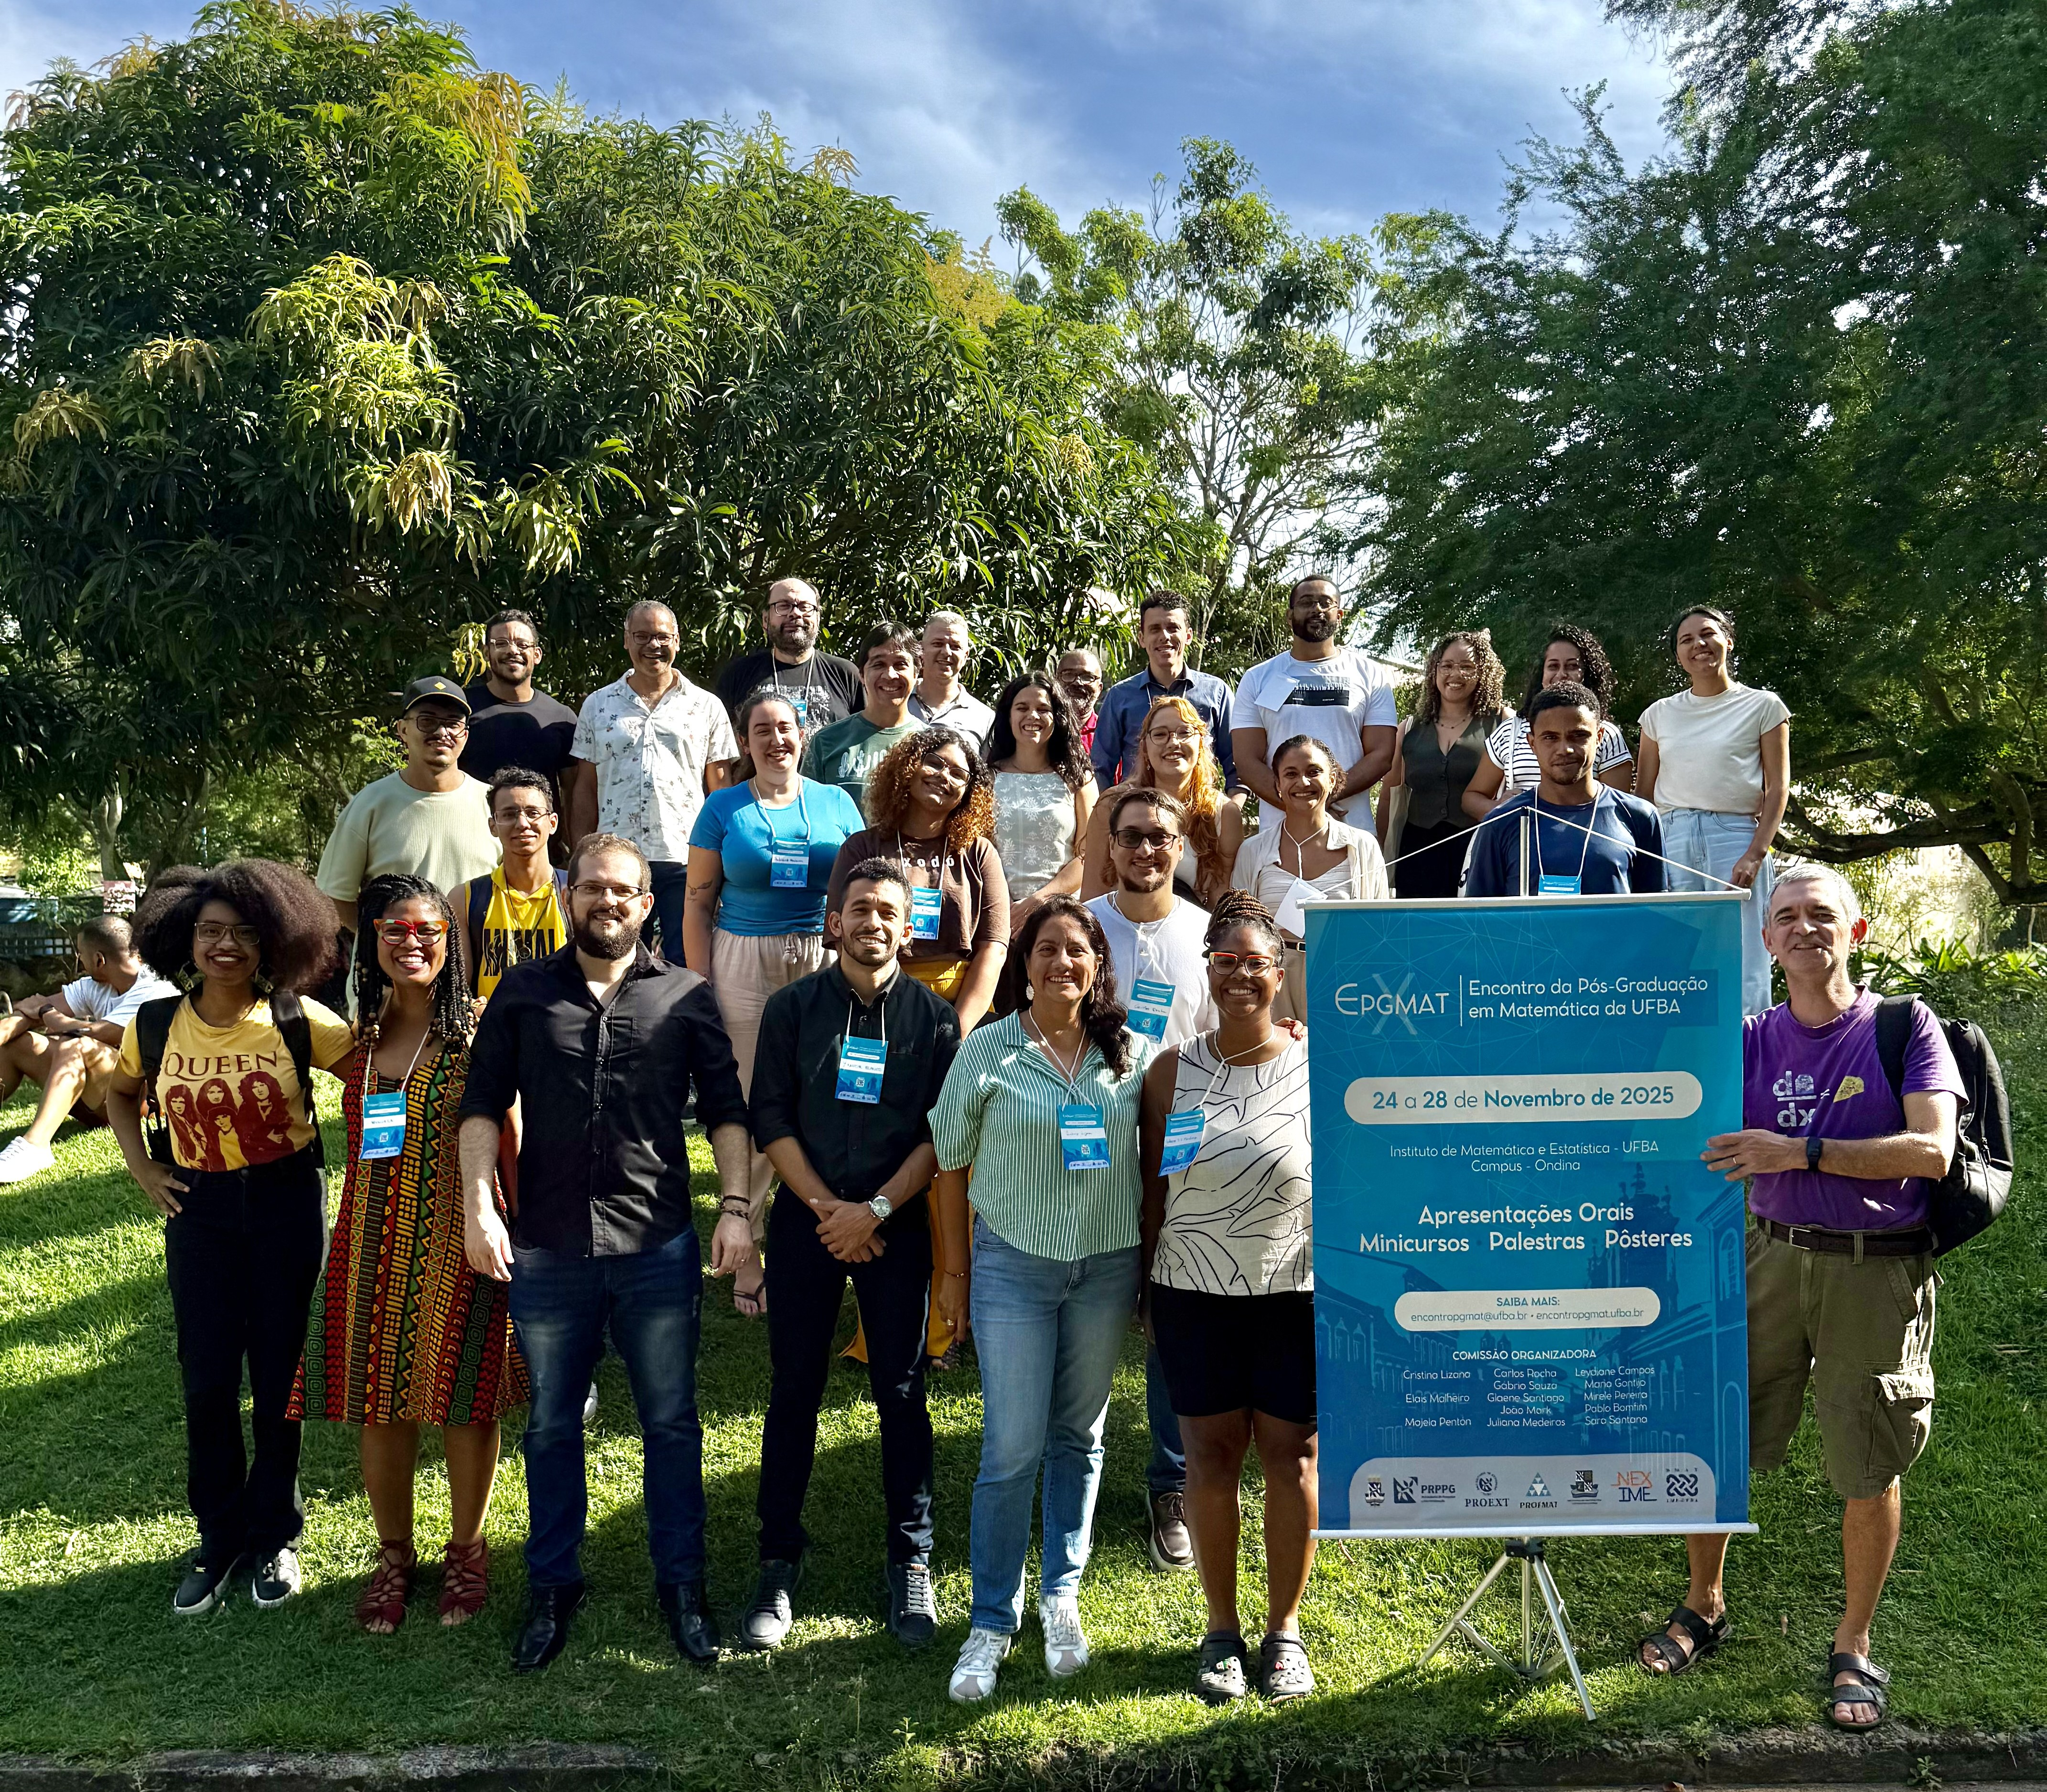
\includegraphics[width=8.5cm]{epgmat1.jpg}
    \caption{Foto de grupo do X EPPGMAT - UFBA.}
 \label{fig:epgmat_foto_grupo}
\end{figure}

Além de um minicurso na área de Sistemas Dinâmicos, a programação de 2025 apresentou uma ampla gama de temas, com palestras, por exemplo, sobre ``Teoria Abstrata dos Modelos: sobre esboços e instituições'', e ``Ferramentas de IA para Aprender e Criar''. As discussões de pesquisa avançadas foram enriquecidas com contribuições de docentes e estudantes da UFBA, e pesquisadores convidados externos, como Keti Tenenblat da UNB, Zaqueu Ramos da UFS e Luciana Salgado da UFRJ.


Um aspecto relevante nesta edição, que reflete uma abordagem de tópicos centrais do ambiente acadêmico atual, foi a inclusão de uma Mesa Redonda intitulada ``Saúde Mental na Pós-Graduação: Ações, Desafios e Caminhos Possíveis'', que levantou discussões sobre o tema e apresentou iniciativas desenvolvidas na UFBA. A mesa contou com a presença das professoras Denise Vieira (Chefe de Gabinete da UFBA) e Martha Macedo (Coordenadora do PSIU-UFBA), que compartilharam ações e desafios na construção de uma universidade mais acolhedora e saudável.

\begin{figure}[htb]
    \centering
    \includegraphics[width=7.5cm]{epgmat_saude.jpg}
    \caption{Mesa redonda sobre saúde mental com as professoras Denise Vieira (Chefe de Gabinete) e Martha Macedo (PSIU-UFBA).}
    \label{fig:epgmat_saude}
\end{figure}

Os estudantes de Doutorado em Matemática da UFBA apresentaram 16 Comunicações Orais, com pesquisas que variaram de ``Caracterização da Semi-Hiperbolicidade via Medida de Máxima Entropia''  a  ``Estimativas de grandes desvios para o passeio aleatório no Toro''. O PROFMAT também contribuiu com duas comunicações orais, e discentes da Graduação e Pós-Graduação tiveram a oportunidade de apresentar suas pesquisas em sessões de Pôsteres.

\begin{figure}[htb]
    \centering
    \includegraphics[width=8.5cm]{epgmat2.jpg}
    \caption{Sessão do PROFMAT no X EPGMAT.}
 \label{fig:epgmat_profmat}
\end{figure}

Em síntese, o X EPGMAT aprofundou a disseminação do conhecimento em Matemática, reforçando o papel de liderança do Programa de Pós-Graduação em Matemática da UFBA, ao mesmo tempo que abordou questões relevantes do ambiente acadêmico atual, como o bem-estar mental dos integrantes dos programas.

Para mais informações sobre o Encontro da Pós-graduação em Matemática da UFBA, acesse \href{https://encontropgmat.ufba.br/}{https://encontropgmat.ufba.br}.

\section{Seminário de Iniciação Científica}

O Seminário de Iniciação Científica do DMAT, que já havia acontecido em 2021 e 2022, em formato online e sob organização do Programa de Pós-Graduação em Matemática da UFBA, foi retomado no primeiro semestre de 2025 por iniciativa dos alunos de graduação que participam de projetos de IC, com apoio da professora Cristina Lizana e do Programa de Pós-Graduação em Matemática. Mais informações sobre as edições anteriores estão disponíveis em \url{https://dgmp.mat.ufba.br/ICmat/seminarioICmat.html}.

%O Seminário de Iniciação Científica do DMAT foi retomado no primeiro semestre de 2025 por iniciativa dos alunos de graduação que participam de projetos de IC, com apoio da professora Cristina Lizana e do Programa de Pós-Graduação em Matemática. A iniciativa já havia sido executada em 2021 e 2022, em formato online e sob a organização pelo Programa de Pós-Graduação em Matemática da UFBA. Mais informações sobre essas edições estão disponíveis em \url{https://dgmp.mat.ufba.br/ICmat/seminarioICmat.html}.

A proposta do seminário é ser um espaço descontraído e colaborativo, desenvolvido pelos estudantes e voltado para eles mesmos, onde cada participante pode apresentar seus tópicos de estudo e compartilhar experiências com colegas. Além de valorizar o trabalho desenvolvido em cada projeto de iniciação científica, o seminário busca estimular a troca de ideias e promover o amadurecimento acadêmico e científico dos alunos.

\begin{figure}[htb]
    \centering
    \includegraphics[width=8.5cm]{ic1.jpg}
    \caption{Primeiro encontro do Seminário de Iniciação Científica em abril de 2025.}
 \label{epgmat}
\end{figure}

Em 2025, os encontros aconteceram quinzenalmente e somaram 12 apresentações. A organização ficou a cargo dos próprios estudantes, sempre com a supervisão da professora Cristina Lizana. No primeiro semestre, os doutorandos Leydiane Campos e Elivan Neri Lima organizaram os encontros junto com o discente da graduação Mateus de Santana. Já no segundo semestre, Samuel Figueiredo (graduação) assumiu a coordenação, com apoio de Tácio Fernandes (mestrado) e novamente Elivan Neri Lima (doutorado).

\begin{figure}[htb]
    \centering
    \includegraphics[width=8.5cm]{ic2.jpg}
    \caption{Último encontro do Seminário de Iniciação Científica em dezembro de 2025.}
 \label{epgmat}
\end{figure}

O seminário seguirá em 2026, trazendo uma nova programação e mantendo o compromisso de fortalecer a integração e o desenvolvimento científico dos estudantes. Fique atento às redes sociais do DMAT!


%%%% BLOCO 2 %%%%

\sepdecorada

%\begin{center}
\noindent {\Large\textbf{\textsc{Integração e Vivência Acadêmica}}}
%\end{center}

\noindent \textit{Voltando o olhar para a nossa comunidade, o ano também foi marcado por projetos de extensão e vivência acadêmica que fortalecem a memória institucional e a formação integral dos nossos estudantes.}

\section{PECMat em 2025: Fortalecendo o Vínculo entre Gerações}

O ano de 2025 marcou um período de intensa articulação para o projeto de extensão PECMat (Egressos dos cursos de Matemática da UFBA), consolidando seu papel fundamental na vida acadêmica do Instituto. O projeto avançou para além do mapeamento de ex-estudantes, transformando-se em um espaço vibrante de reconhecimento de trajetórias e troca de experiências.

\begin{figure}[htb]
    \centering
    \includegraphics[width=8.5cm]{PECMat1.jpg}
    \caption{Ex-alunos e Diretores do IME, no Bate-Papo com a Prof\superau.\  Célia Gomes.}
    \label{fig:pecmat1}
\end{figure}

Os Bate-Papos com Egressos apresentaram um panorama inspirador, conectando gerações. Tivemos a participação de lideranças institucionais, como o atual Diretor do IME, Prof.\  Kleyber Mota, e a Prof\superau.\  Célia Gomes (aposentada), ex-diretora do antigo Instituto de Matemática, que compartilharam suas visões sobre a gestão e a evolução da carreira acadêmica.

Além da gestão, o projeto destacou a pesquisa em Educação Matemática e a prática docente. Egressos como a Prof\superau.\  Jamille Vilas Bôas (IFBA/Salvador) trouxeram debates sobre o ensino, enquanto o egresso Paulo Malta (IFBA/Porto Seguro) ministrou uma oficina prática sobre demonstrações do Teorema de Pitágoras, integrando formação técnica e compromisso extensionista.

\begin{figure}[htb]
    \centering
    \includegraphics[width=8.5cm]{PECMat2.jpg}
    \caption{Oficina PECMat do LEMA com estudantes do IFBA.}
    \label{fig:pecmat2}
\end{figure}

Um momento de grande emoção foi a valorização da memória institucional, com a homenagem à Prof\superau.\  Elinalva Vergasta (Lina), figura central na história do Laboratório de Ensino (LEMA), atualmente aposentada. O egresso Fellipe Antônio conduziu o debate ``Minha Vida Como Rato de Laboratório'', destacando o impacto pedagógico e afetivo do LEMA na formação de gerações.

Outro marco foi o encontro com o Prof.\  José Fernandes (aposentado), realizado durante o XVIII EMAT. O bate-papo revisitou sua trajetória e contribuições decisivas para a pós-graduação, promovendo um valioso cruzamento entre docentes aposentados, professores na ativa e estudantes.

%\begin{figure}[htb]
%    \centering
%    \includegraphics[width=8.5cm]{PECMat3.jpg}
%    \caption{Encontro de gerações no Bate-Papo PECMat com o Prof.\  Zé Fernandes.}
%    \label{fig:pecmat3}
%\end{figure}

A conexão com o presente também se deu nas recepções realizadas no início de cada semestre do ano, onde o público, especialmente os calouros, foi acolhidos com os bate-papos intitulados ``A minha vida tem lógica!'' e ``A dinâmica caótica para se tornar um matemático'', ministrados, respectivamente, pelos professores Darllan Pinto (Chefe do DMAT) e Kleyber Mota. 

Com uma equipe dedicada de docentes e estudantes atuando na execução das atividades, sob a coordenação da Prof\superau.\  Elaís Cidely, as discussões abordadas também se voltaram para temas como inclusão de meninas na Matemática, vivências e trajetórias nas olimpíadas de Matemática, empreendedorismo, desafios emocionais da carreira, entre outros. 

%A conexão com o presente se deu nas recepções aos novos semestres. Com temas como ``A minha vida tem lógica!'' e ``A dinâmica caótica para se tornar um matemático'', os calouros foram acolhidos pelo Prof.\  Darllan Pinto (Chefe do DMAT) e Kleyber Mota, que discutiram desafios, planejamento de carreira e a construção da identidade profissional.

%A execução das atividades contou com uma equipe dedicada de docentes e estudantes sob a coordenação da Prof\superau.\  Elaís Cidely. Para ampliar o acesso, os encontros foram gravados e disponibilizados no canal do DMAT no YouTube.

\begin{figure}[htb]
    \centering
    \includegraphics[width=8.5cm]{PECMat4.jpg}
    \caption{Equipe PECMat atual.}
    \label{fig:pecmat4}
\end{figure}

Para ampliar o acesso, os encontros foram gravados e disponibilizados no canal do \href{https://www.youtube.com/c/depmatufba}{DMAT} no YouTube.
Para mais informações, acesse o perfil no Instagram: \href{https://www.instagram.com/pecmatufba}{@pecmatufba}.


\section{Seminário Café Cultural}

O Seminário Café Cultural, coordenado pelos professores Cristina Lizana e Roberto Sant'Anna, manteve sua agenda ativa e diversificada em 2025, reafirmando seu compromisso com a formação complementar e o debate multidisciplinar.

\begin{figure}[htb]
    \centering
    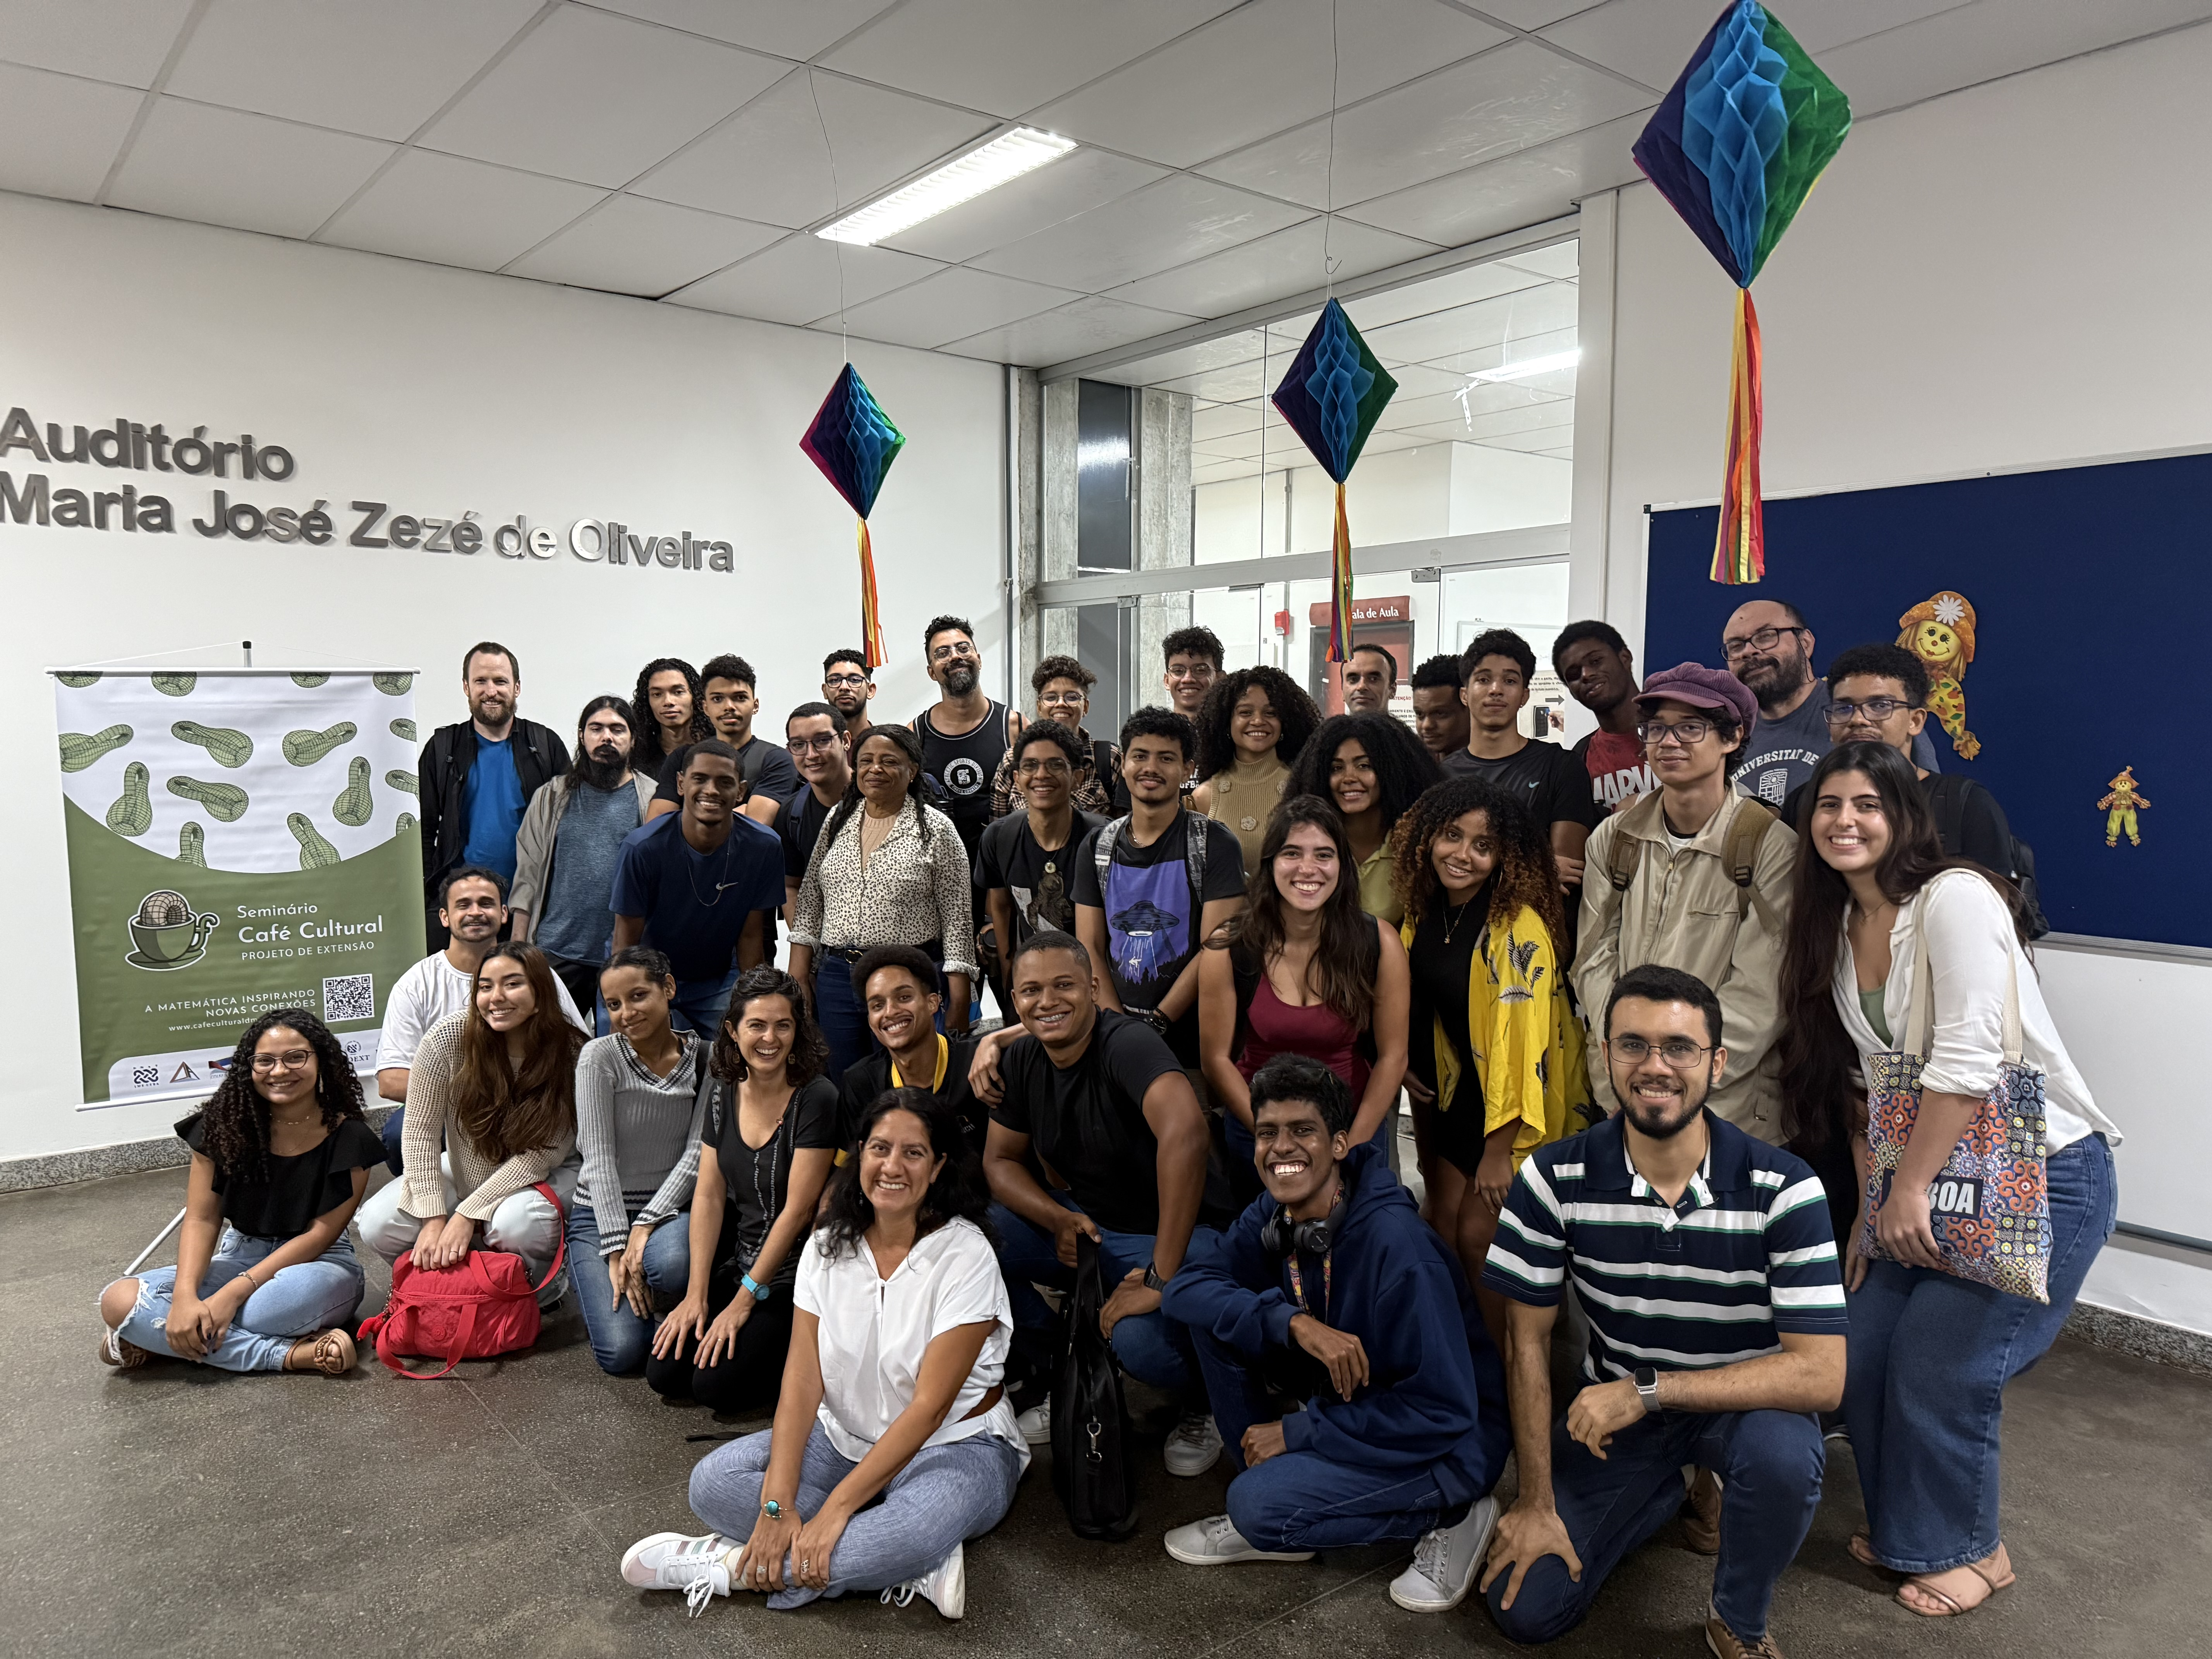
\includegraphics[width=8.5cm]{cafe1.jpg}
    \caption{Prof\superau.\  Vanessa Barros (DMAT) no Seminário Café Cultural.}
    \label{fig:svmc_equipe}
\end{figure}

O ano iniciou com uma edição especial em janeiro, recebendo os professores visitantes Antonio Caminha (UFC) e Ana Paula Chaves (UFG) para uma sessão dupla sobre Geometria e Teoria dos Números. Outro momento de destaque foi a celebração do ``May 12 - Celebrating Women in Mathematics'', que contou com a exibição presencial do documentário sobre a vida da medalhista Fields, Maryam Mirzakhani.

A programação de 2025 caracterizou-se por um forte diálogo com outras áreas, promovendo mesas redondas e palestras que integraram a Matemática com a Biologia (em parceria com o IBIO-UFBA), a Física (Projeto Física Fora da Caixinha) e a Educação Inclusiva (Projeto Modelando Matemática/ICTI). O seminário também trouxe respostas lúdicas para questionamentos clássicos, com destaque para a palestra ``Professora, para que serve a matemática?'', ministrada pela Prof\superau.\  Vanessa Barros. Nela, a docente explorou a geometria e o cálculo no cotidiano, analisando desde o formato de batatas {\it chips} até o design ideal de copos para conservar a temperatura de bebidas.

%A programação de 2025 caracterizou-se por um forte diálogo com outras áreas, promovendo mesas redondas e palestras que integraram a Matemática com a Biologia (em parceria com o IBIO-UFBA), a Física (Projeto Física Fora da Caixinha) e a Educação Inclusiva (Projeto Modelando Matemática/ICTI). O seminário também fomentou discussões internas importantes, abordando o uso da História da Matemática em sala de aula e o papel da Iniciação Científica na formação discente.

\begin{figure}[htb]
    \centering
    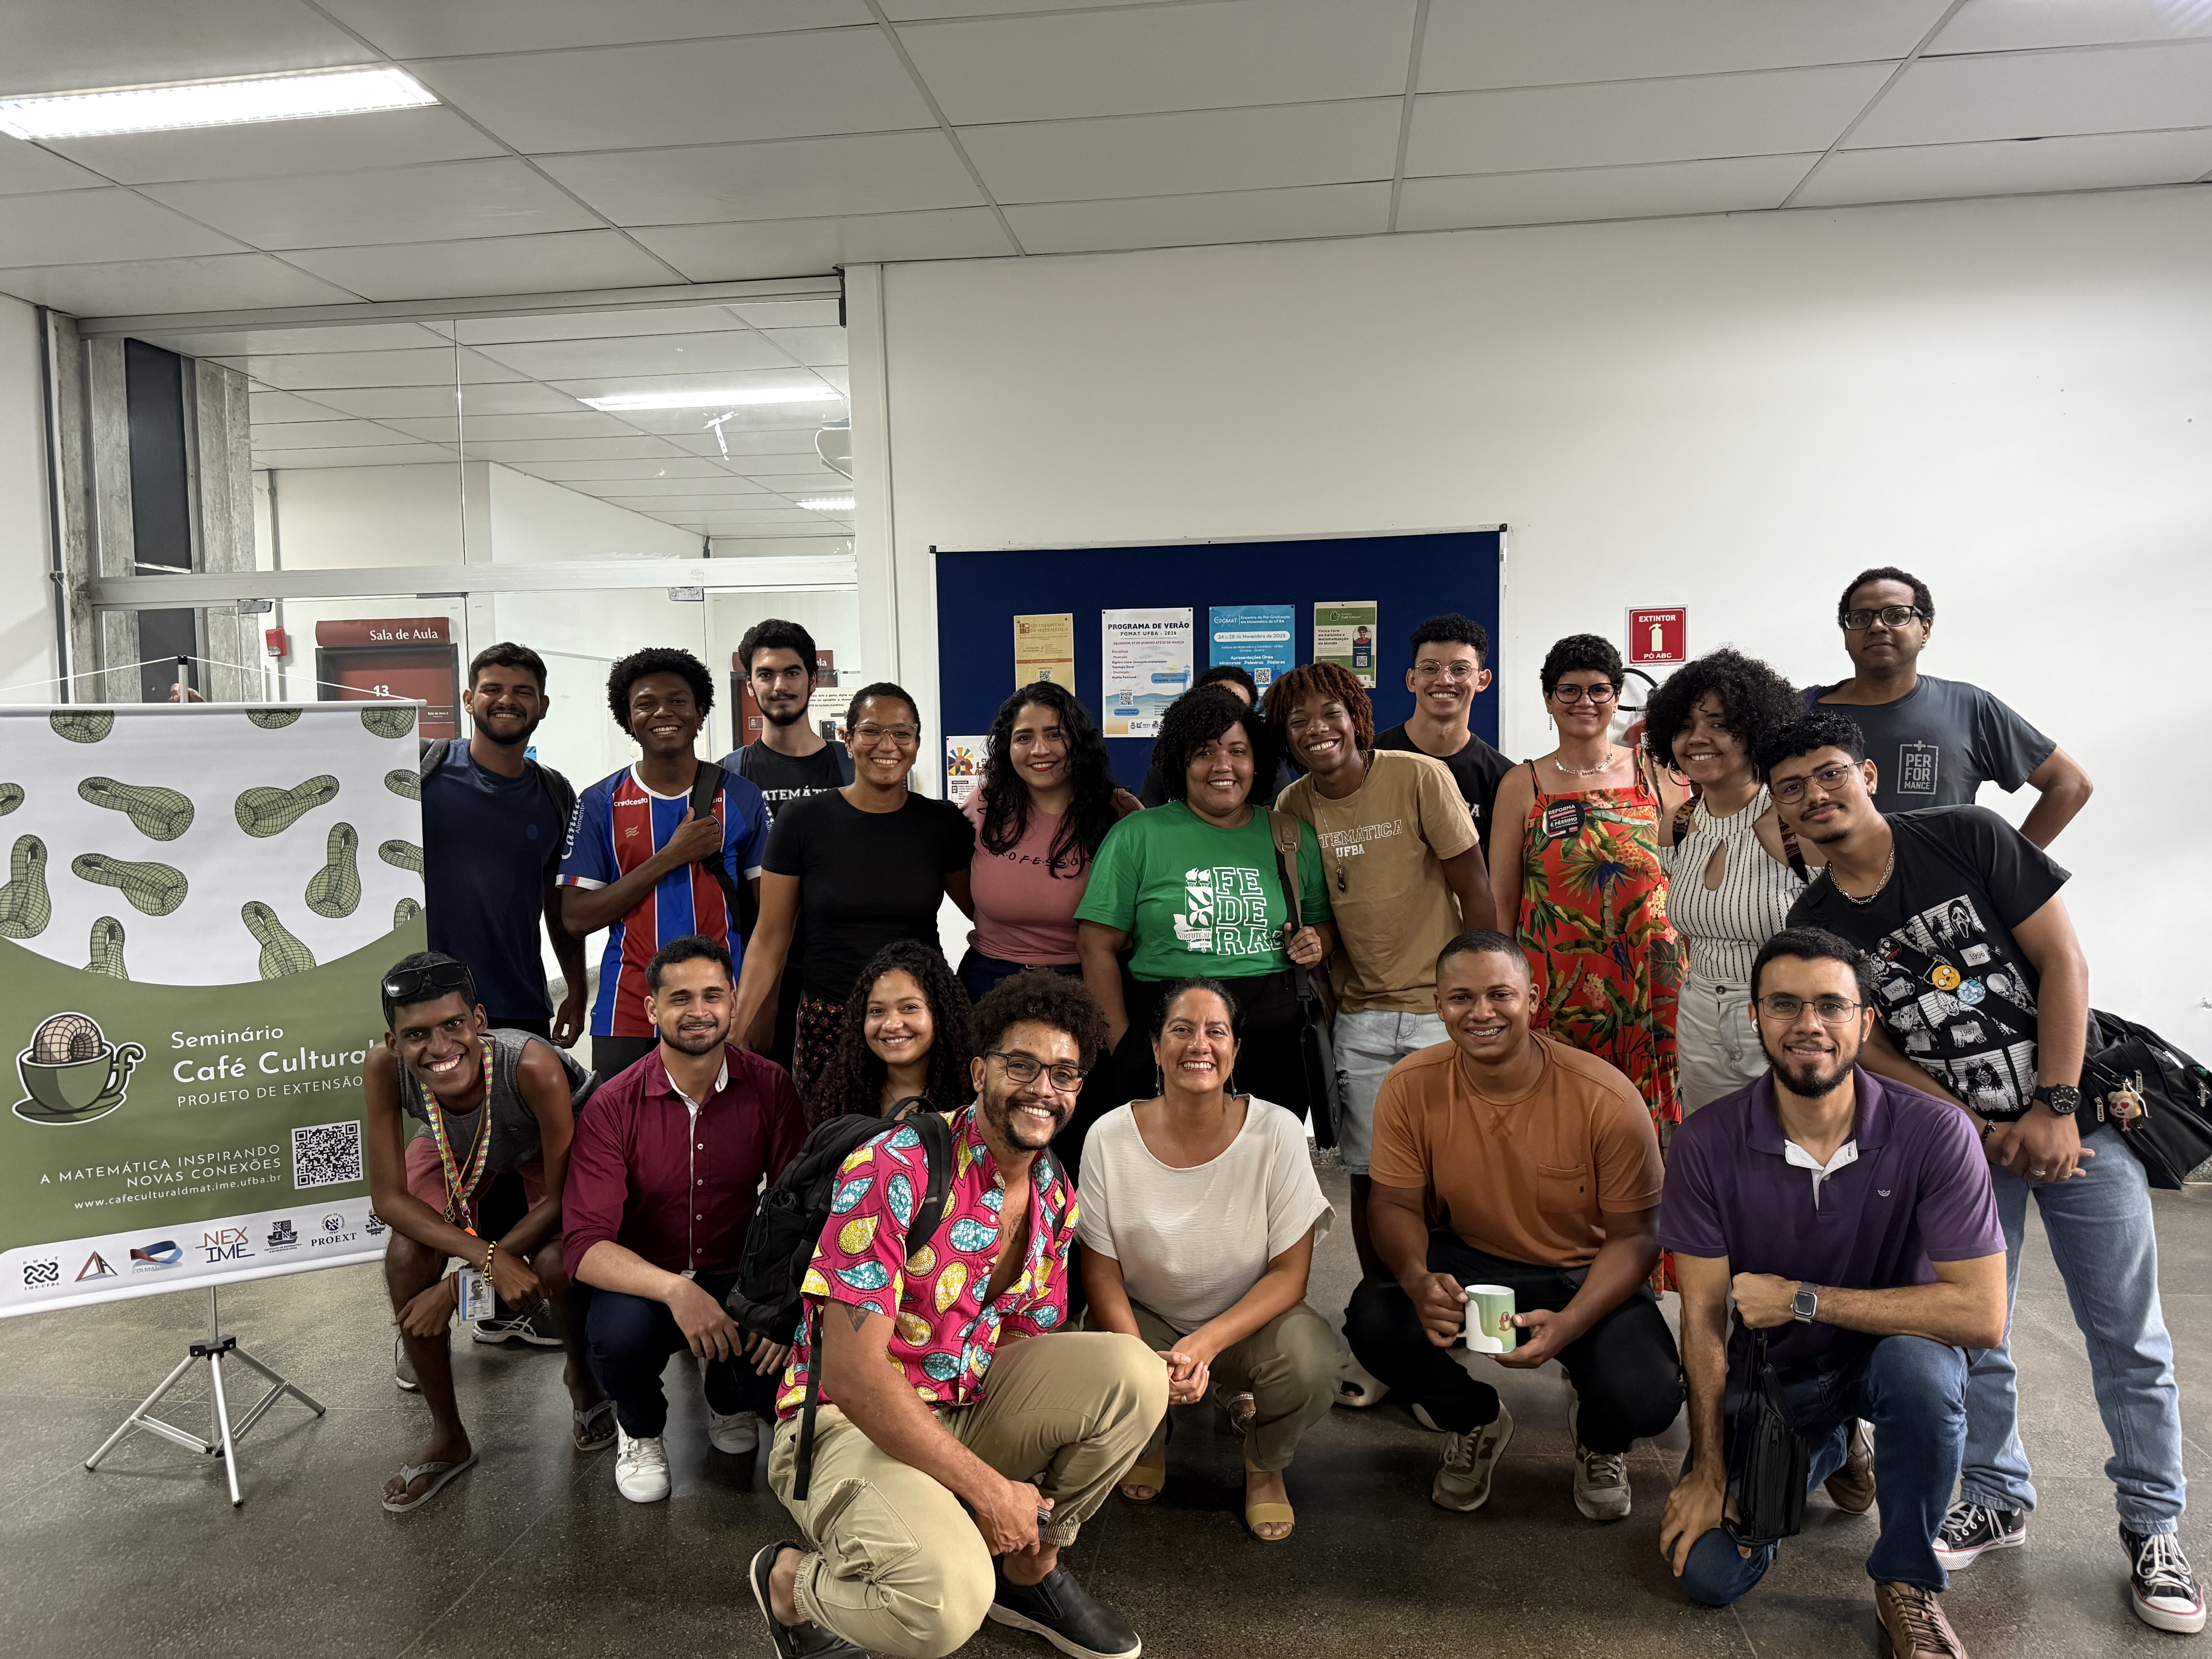
\includegraphics[width=8.5cm]{cafe_fisica.jpg}
    \caption{Prof.\   Alexandre Barbosa (IF) no Seminário Café Cultural.}
    \label{fig:svmc_equipe}
\end{figure}

As atividades ocorreram no Auditório do IME, muitas com transmissão simultânea, garantindo o acesso ampliado ao conteúdo. Para mais informações e acesso às gravações, visite \href{http://www.cafeculturaldmat.ime.ufba.br/}{http://www.cafeculturaldmat.ime.ufba.br}.


\section{I Seminário de Visualização e Matemática Computacional}

Com a provocação ``Como podemos enxergar a matemática?'', ocorreu no dia 09 de julho de 2025 o I Seminário de Visualização e Matemática Computacional (SVMC). O evento marcou a primeira grande ação pública do recém-criado Núcleo de Estudos em Matemática Pura e Aplicada (NEMPA).

% Foto 1: Palestra Vinícius
\begin{figure}[htb]
    \centering
    \includegraphics[width=8.5cm]{svmc_vinicius.jpg}
    \caption{Prof.\  Vinícius Mello apresenta um panorama histórico da visualização matemática.}
    \label{fig:svmc_palestra}
\end{figure}

Sob a coordenação do Prof.\  Roberto Sant'Anna e com apoio da equipe técnica do núcleo, o seminário reuniu mais de 60 participantes no Auditório do IME. A programação contou com palestras ministradas pelos professores do DMAT Vinícius Mello, Carlos Siqueira, Perfilino Júnior e Roberto Sant'Anna, oferecendo um panorama abrangente da área.

As discussões transitaram desde uma perspectiva histórica da visualização matemática até a geometria fractal da natureza e o processamento de imagens digitais, culminando na demonstração prática de animações matemáticas usando a biblioteca Manim em Python. O sucesso de público demonstrou o potencial desta área na UFBA, estabelecendo as bases para futuros projetos de computação científica e divulgação visual.

% Foto 2: Equipe
\begin{figure}[htb]
    \centering
    \includegraphics[width=8.5cm]{svmc_equipe.jpg}
    \caption{Palestrantes e equipe de organização do I SVMC no Auditório do IME.}
    \label{fig:svmc_equipe}
\end{figure}


\section{XIX Encontro de Matemática da UFBA (EMAT)}

Encontros de pesquisa de Matemática são comuns e muito abrangentes, tendo como público alvo professores, pesquisadores e alunos de pós-graduação. Tão importantes quanto são os eventos voltados para aqueles que estão iniciando sua vida acadêmica na matemática em cursos de graduação, seja no bacharelado ou em licenciaturas. Para tanto, a 19\textsuperscript{\underline{a}} edição do Encontro de Matemática (EMAT) aconteceu nos dias 10 a 14 de novembro de 2025.

\begin{figure}[htb]
    \centering
    \includegraphics[width=8.5cm]{emat1.jpg}
    \caption{Organizadores e participantes do XIX EMAT.}
    \label{fig:svmc_equipe}
\end{figure}

O evento tem como finalidade divulgar e discutir os cursos de matemática da UFBA e de outras instituições. Esta edição contou com uma vasta programação nos três turnos (manhã, tarde e noite), permitindo que os alunos matriculados em cursos noturnos também tivessem oportunidade de participar. 

 Com cerca de 100 participantes credenciados até o terceiro dia de evento, a programação ofereceu uma imersão de aproximadamente 9 horas diárias de atividades. No total, foram realizadas 17 palestras, 3 minicursos, além de 5 mesas-redondas, 2 oficinas e sessões de pôsteres para a exposição de trabalhos científicos, possibilitando a troca de experiências acadêmicas, o debate de temas atuais da matemática e reflexões sobre pesquisa e formação docente e também reforçando a relevância do EMAT para a formação acadêmica e científica dos participantes.

 \begin{figure}[htb]
    \centering
    \includegraphics[width=8.5cm]{emat2.jpg}
    \caption{Foto de grupo após palestra da Prof\superau.\  Vanessa Barros durante a programação do XIX EMAT.}
    \label{fig:emat_vanessa}
\end{figure}

A organização desta edição foi inteiramente formada por alunos do IME, mobilizando um total de 43 estudantes em diversas frentes de trabalho, sob a liderança de uma comissão central composta pelos discentes Amanda dos Santos, Clara Rios, Gabriel Siron, Jay Victor Cintra, João Victor Delgado, Larissa de Jesus Mota e Sergio Samuel Figueiredo.  Para sua realização, o EMAT contou com o apoio crucial da PROEXT (Pró-Reitoria de Extensão), além do suporte do Diretório Acadêmico, do Departamento de Matemática e de doações de 29 professores da unidade.

%A organização desta edição foi inteiramente formada por alunos do IME, a coordenação do evento foi liderada por uma comissão central composta pelos discentes Amanda dos Santos, Clara Rios, Gabriel Siron, Jay Victor Cintra, João Victor Delgado, Larissa de Jesus Mota e Sergio Samuel Figueiredo, mobilizando um total de 43 estudantes em diversas frentes de trabalho. Para sua realização, o EMAT contou com o apoio crucial da PROEXT (Pró-Reitoria de Extensão), além do suporte do Diretório Acadêmico, do Departamento de Matemática e de doações de 29 professores da unidade.

\begin{figure}[htb]
    \centering
    \includegraphics[width=8.5cm]{cafe_emat.jpg}
    \caption{Mesa redonda promovida pelo Seminário Café Cultural no XIX EMAT.}
    \label{fig:svmc_equipe}
\end{figure}

Durante o evento, ocorreram em paralelo edições especiais de outros projetos da casa: o \textbf{Café Cultural}, com uma mesa redonda formada por alunos de graduação e pós-graduação discutindo os primeiros passos na pesquisa matemática; e o \textbf{PECMat}, em que o Prof.\  José Fernandes teve oportunidade de compartilhar sua jornada pessoal e profissional no mundo da Academia e da Matemática.

Acompanhe as redes sociais do evento em \href{https://www.instagram.com/ematufba/}{@ematufba} para ficar em dia com as edições futuras!



\section{Seminários de Educação Matemática} 
Em junho de 2025, o grupo dos professores da área de Educação Matemática do Instituto de Matemática e Estatística da UFBA (IME/UFBA), Graça Dominguez, Elias Santiago, Kátia Lima e Diogo Rios, deu início ao projeto de ensino e pesquisa intitulado \textit{Seminários de Educação Matemática}. A iniciativa é direcionada para estudantes da graduação em Licenciatura em Matemática, profissionais da Educação Básica, estudantes de outros cursos de graduação ou pós-graduação interessados em estabelecer relações com o tema e compreender o que é ``fazer ciência'' nesse campo científico.

\begin{figure}[htb]
    \centering
    \includegraphics[width=7.5cm]{EduMat.jpeg}
    \caption{Coordenadores do Seminário de Educação Matemática.}
 \label{epgmat}
\end{figure}

O projeto configura-se como um espaço colaborativo para estudos e reflexões sobre as diversas subáreas da Educação Matemática. Sob a mediação dos professores coordenadores, o grupo promove  estudos dirigidos, minicursos e momentos de socialização de saberes. Mais que um espaço para difusão de trabalhos da área, o seminário funciona como um fomentador de novas pesquisas, ao suscitar o interesse dos participantes pelas temáticas abordadas, as quais podem fundamentar futuros trabalhos e propostas de pesquisa em suas trajetórias acadêmicas.

Nesses primeiros meses de existência, o grupo estabeleceu uma rotina de reuniões semanais, abordando tópicos fundamentais. Entre os debates realizados, destacam-se os materiais curriculares, o fazer docente, a trajetória histórica do currículo de Matemática no Brasil e a institucionalização da Educação Matemática como um campo científico no país. O projeto também se mantém atento às transformações tecnológicas contemporâneas, tendo discutido as complexas relações entre a Inteligência Artificial e o ensino de Matemática.

Para 2026, a coordenação planeja expandir o alcance das discussões e debates. Entre as metas estabelecidas, está o convite a pesquisadores externos para ministrarem oficinas e/ou minicursos. O objetivo é oferecer perspectivas complementares e aprofundar os temas sugeridos pelos próprios participantes, consolidando o seminário como um polo dinâmico de formação e investigação científica na área de Educação Matemática no Departamento de Matemática da UFBA.

Para mais informações sobre os Seminários, acesse o instagram do DMAT: \href{https://www.instagram.com/dmatufba?igsh=MXJ0NDVjaThwc2IwMQ==}{@dmatufba}.


%%%% BLOCO 3 %%%%

\sepdecorada

%\begin{center}
\noindent {\Large\textbf{\textsc{Diálogos com Escola e Sociedade}}}
%\end{center}

\noindent \textit{Para além dos muros da universidade, o departamento ampliou seu impacto social, levando a matemática de forma lúdica, inclusiva e desafiadora para centenas de jovens da educação básica, promovendo a diversidade e a história na descolonização do conhecimento.}

\section{28\superau\  Semana Olímpica da OBM em Salvador}

Entre os dias 26 de janeiro e 2 de fevereiro de 2025, Salvador tornou-se a capital nacional da matemática ao sediar a 28\superau\  Semana Olímpica. O evento, promovido pela Associação da Olimpíada Brasileira de Matemática (AOBM), reuniu centenas de estudantes medalhistas da OBM e do Torneio Meninas na Matemática (TM²) de todo o Brasil para uma imersão de alto nível.

Embora seja um evento nacional, a realização desta edição contou com o suporte logístico e organizacional fundamental do Programa de Extensão Matemática Olímpica da UFBA. Sob a coordenação do Prof.\  Samuel Feitosa (DMAT-UFBA) e com o apoio local do professor Roberto Sant'Anna, a equipe de extensão --- incluindo docentes e discentes como Carlos Rocha, Sara Sousa e Elaís Cidely --- garantiu o sucesso das atividades.

\begin{figure}[htb]
    \centering
    \includegraphics[width=8.5cm]{semana_equipe_local.jpg}
    \caption{Integrantes do Programa de Extensão Matemática Olímpica (Elaís Cidely, Carlos Rocha e Sara Sousa) na organização do evento.}
    \label{fig:semana_equipe}
\end{figure}

A programação incluiu aulas avançadas, palestras de orientação acadêmica e a tradicional ``Vingança Olímpica'', uma competição divertida onde os alunos criam problemas para os professores resolverem. O encerramento foi marcado pela Cerimônia de Premiação, que contou com a presença de autoridades da matemática brasileira, como o Prof.\  Carlos Gustavo Moreira (Gugu), e do Diretor do IME-UFBA, Prof.\  Kleyber Mota.

\begin{figure}[htb]
    \centering
    \includegraphics[width=8.5cm]{semana_mesa.jpg}
    \caption{Mesa da cerimônia de premiação com a presença dos professores Carlos Moreira (Gugu), Kleyber Mota, Edmilson Motta e Luíze D'Urso, bem como Carolina da Costa (Instituto Stone) e o vice-presidente da SBM Daniel Pellegrino.}
    \label{fig:semana_mesa}
\end{figure}

O evento também promoveu um rico intercâmbio entre educadores. Momentos de fala conjunta, como o protagonizado pelo coordenador Samuel Feitosa ao lado de Carlos Gomes (UFRN), Rogério Steffenon (UNISINOS), reforçaram a importância da colaboração interinstitucional para o fortalecimento das olimpíadas no país.

\begin{figure}[htb]
    \centering
    \includegraphics[width=8.5cm]{semana_coordenacao.jpg}
    \caption{Prof.\  Samuel Feitosa (UFBA) em atividade com Carlos Gomes (UFRN) e Rogério Steffenon (UNISINOS).}
    \label{fig:semana_samuel}
\end{figure}

Inspirados pelo sucesso deste encontro e visando fomentar ainda mais a cultura olímpica no Estado, o DMAT-UFBA anuncia a criação da \textbf{1\superau\  Semana Olímpica da UFBA}, prevista para fevereiro de 2026. O novo evento terá como foco a integração e o incentivo aos talentos da Bahia, consolidando o trabalho que vem sendo realizado pelos interessados na área em todo o Estado.

\section{Aulões Olímpicos: Superando Desafios em Matemática}

Ao longo de 2025, o Instituto de Matemática e Estatística (IME-UFBA) abriu suas portas para receber centenas de estudantes da Educação Básica por meio da ação de extensão Aulão Olímpico: Superando Desafios em Matemática. Coordenada pelo Prof.\  Roberto Sant'Anna, a iniciativa consolidou-se como uma ponte vital entre a escola e a universidade, tendo como objetivo principal não apenas o treinamento técnico, mas a desmistificação do ambiente acadêmico e o fortalecimento da cultura olímpica em escolas públicas de Salvador e Região Metropolitana.

% Foto 1: Aula
\begin{figure}[htb]
    \centering
    \includegraphics[width=8.5cm]{aulao_classe.jpg}
    \caption{Estudante de graduação do Programa de Extensão ministrando aula para alunos da rede pública.}
    \label{fig:aulao_classe}
\end{figure}

Diferente de treinamentos tradicionais focados apenas na repetição, os encontros se destacaram pelo caráter multidisciplinar e humanista. A programação integrou o rigor da Matemática com atividades culturais inovadoras, como a parceria com o Projeto de Extensão Cineclube de História da Matemática e a realização de oficinas de teatro. Estas últimas visaram o desenvolvimento da oratória e a desinibição, competências essenciais para a formação integral dos jovens talentos.

A diversidade de atividades incluiu também uma imersão científica durante a Semana Nacional de Ciência e Tecnologia (SNCT), onde os estudantes puderam visitar o Planetário da UFBA, conectando a matemática à astronomia e expandindo seus horizontes científicos.

% Foto 2: Planetário
\begin{figure}[htb]
    \centering
    \includegraphics[width=8.5cm]{aulao_planetario.jpg}
    \caption{Visita ao Planetário da UFBA: integrando ciência e cultura na formação dos estudantes.}
    \label{fig:aulao_planetario}
\end{figure}

Um ponto alto e distintivo do projeto foi a abordagem socioemocional. Reconhecendo que o desempenho acadêmico está atrelado ao bem-estar mental, diversas edições contaram com palestras de psicólogos, como a realizada em outubro com a psicóloga Taíris Araújo. O foco na gestão da ansiedade pré-prova preparou os alunos não apenas intelectualmente, mas emocionalmente para os desafios de competições como a OBMEP e o ENEM.

% Foto 3: Psicóloga
\begin{figure}[htb]
    \centering
    \includegraphics[width=8.5cm]{aulao_psico.jpg}
    \caption{Aulão inaugural com intervenção sobre gestão emocional e ansiedade, conduzida pela psicóloga Taíris Araújo.}
    \label{fig:aulao_psico}
\end{figure}

O ano encerrou com uma expansão ambiciosa das fronteiras do projeto: a organização da ``Seleção Baiana'' para a olimpíada internacional \textit{Formula of Unity}, em parceria com a Universidade de São Petersburgo (Rússia). Esta iniciativa inédita permitiu que estudantes da rede pública baiana tivessem contato com problemas desafiadores de padrão internacional, colocando a Bahia no mapa da matemática global nesta área.

O projeto contou com a participação engajada de diversas instituições, como o Colégio da Polícia Militar (unidades Candeias e Dendezeiros), o Colégio Estadual Central e o Colégio Estadual Anna Junqueira Ayres Tourinho - CEAJAT (São Francisco do Conde), reafirmando o IME-UFBA como um espaço de pertencimento e transformação social para a juventude baiana.

Para acompanhar a agenda dos próximos aulões, acesse \href{https://www.instagram.com/mat.olimpica}{@mat.olimpica}.


\section{Cerimônias de Premiação: Celebrando Talentos}

O ano de 2025 foi marcado por grandes celebrações do mérito acadêmico, reafirmando o compromisso da UFBA e do DMAT com a valorização da ciência na Educação Básica. Mais do que a entrega de medalhas, estes eventos representaram o ápice de um trabalho contínuo de inclusão e descoberta de talentos, promovendo o encontro emocionante entre a universidade, as escolas públicas e as famílias dos estudantes.

% Foto 1: Plateia OBMEP
%\begin{figure}[htb]
%    \centering
%    \includegraphics[width=8.5cm]{obmep_plateia.jpg}
%    \caption{Alunos premiados aguardam a chamada durante a Cerimônia Regional da OBMEP.}
%    \label{fig:obmep_plateia}
%\end{figure}

No dia 22 de julho, o Salão Nobre da Reitoria sediou a Cerimônia Regional da 19\superau\  Olimpíada Brasileira de Matemática das Escolas Públicas (OBMEP) - Regional BA01. O evento solene, sob coordenação do Prof.\  Roberto Sant'Anna, contou com a presença do Vice-Reitor em exercício, Prof.\  Penildon Silva Filho, e diretores da universidade. A presença massiva da comunidade escolar celebrou um resultado expressivo da nossa região, que acumulou 77 medalhas nacionais e 229 medalhas regionais, refletindo a capilaridade e a força do ensino de matemática na Bahia.

% Foto 3: Mesa Diretora
\begin{figure}[htb]
    \centering
    \includegraphics[width=8.5cm]{obmep_mesa.jpg}
    \caption{Mesa diretora da solenidade na Reitoria da UFBA.}
    \label{fig:obmep_mesa}
\end{figure}

Para além dos números, a cerimônia buscou integrar diferentes formas de conhecimento. Um destaque especial desta edição foi a união entre Arte e Ciência. A solenidade foi abrilhantada por apresentações culturais do Maestro José Maurício Brandão (piano) e da soprano Gisele Nino, que trouxeram leveza e sofisticação ao ambiente, emocionando o público presente e mostrando que a matemática dialoga com todas as esferas da cultura humana.

% Foto 2: Arte (Música)
\begin{figure}[htb]
    \centering
    \includegraphics[width=8.5cm]{obmep_arte.jpg}
    \caption{Apresentação artística do Maestro José Maurício Brandão e da soprano Gisele Nino.}
    \label{fig:obmep_arte}
\end{figure}

Encerrando o ciclo anual, em 04 de dezembro, ocorreu a premiação da 9\superau\  Olimpíada de Matemática do Estado da Bahia (OMEBA). Organizada pelos professores Henrique Barbosa, Roberto Sant'Anna e Samuel Feitosa, a cerimônia reuniu estudantes de diversas regiões do Estado, da capital ao interior. Foram premiados 11 medalhistas de ouro, 20 de prata e 33 de bronze. Este evento consolidou a competição como uma referência de excelência estadual e um incentivo fundamental para que os jovens talentos baianos, muitas vezes descobertos em escolas distantes dos grandes centros, percebam a UFBA como sua futura casa.

% Foto 4: Medalhas OMEBA
\begin{figure}[htb]
    \centering
    \includegraphics[width=8.5cm]{omeba_medalhas.jpg}
    \caption{Entrega de medalhas aos estudantes destaque na 9\superau\  OMEBA.}
    \label{fig:omeba_entrega}
\end{figure}

\section{Coletivo Ondjango Asili}

O coletivo Ondjango Asili, braço do projeto de extensão Jogos Africanos e Ensino de Matemática, do DMAT, é coordenado pela Prof\superau.\  Simone Moraes e integrado por estudantes de graduação da UFBA e professores da Educação Básica. Em 2025, reafirmou seu protagonismo na promoção de um ensino de Matemática inclusivo e antirracista. Reconhecido por suas ações significativas na descolonização do ensino de Matemática, o coletivo manteve sua filosofia de criar espaços de (re)união, troca e criação, utilizando jogos e elementos culturais africanos para fundamentar práticas pedagógicas no contexto da Lei 10.639/03.

Após a aprovação do projeto Ananse --- Tecendo sabedoria na matemática com jogos e elementos culturais africanos, em dezembro de 2024 pelo edital Matemática nos finais do Ensino Fundamental do Itaú Social, também coordenado pela professora Simone, o coletivo iniciou o ano promovendo a Exposição dostrabalhos criados na ACCS --- Cultura e Jogos Africanos no Ensino da Matemática. Na ocasião, os estudantes apresentaram os trabalhos por eles desenvolvidos e os participantes tiveram a oportunidade conhecer e
experimentá-los.


Em maio e junho, foram promovidas as Oficinas Ananse --- Tecendo Sabedoria com Matemática, no contexto do projeto do Itaú Social, em diversas escolas de Salvador, Lauro de Freitas e Camaçari. Nas atividades, os estudantes tiveram a oportunidade de explorar conceitos matemáticos de forma lúdica e conectada à ancestralidade africana, por meio de jogos e curiosidades africanas.

% FOTO DA OFICINA NA ESCOLA (Retrato, altura travada)
\begin{figure}[htb]
    \centering
    \includegraphics[height=6.0cm]{simone_vidanova.jpg}
    \caption{Prof\superau.\  Simone Moraes e equipe da Escola Municipal de Vida Nova (Lauro de Freitas) durante a realização das Oficinas Ananse.}
    \label{fig:simone_vidanova}
\end{figure}


Em julho, o coletivo recebeu a equipe do Itaú Social para uma série de atividades no IME-UFBA, em que foram realizadas oficinas de Geometria Sona e jogos como Mbomge e Unxantathu, contando com a participação de 110 estudantes e professores da rede pública. As atividades dessa visita foram documentadas em vídeo (\url{https://youtu.be/Ijp9eACGMg8}) e na coletânea de projetos (\url{https://encurtador.com.br/ebook_itau}), disponíveis online.



\begin{figure}[htb]
    \centering
    \includegraphics[height=6.0cm]{simone_itau.jpg} 
    \caption{A docente com Alexandre Moreira (Itaú Social) durante a premiação no Rio de Janeiro.}
    \label{fig:simone_itau}
\end{figure}

O coletivo também marcou presença em importantes fóruns científicos e educativos, como o V COPENE Nordeste --- ministrando a oficina ``Nea onnim no sua a, ohu'' (Aquele que não sabe, pode aprender), e o Encontro Regional da OBMEP em Salvador, no qual apresentou a Oficina Ananse e os instrutores tiveram a rica experiência de trabalhar com estudantes que se mostraram surpresos e curiosos sobre as informações acerca da cultura africana.

No mês de novembro, afim de promover atividades unindo conhecimento, matemática e diversão, o coletivo realizou novas visitas a escolas aplicando uma oficina de construção de jogos da família Mancala, assim como as oficinas criadas pelos estudantes na disciplina ACCS.


%Para fechar o ciclo anual de atividades do coletivo, foi realizada, no dia 28 de novembro, a 3\superau\  Black Math Friday. Conectado à filosofia Sankofa, que ensina a importância de olhar para o passado para construir o futuro, o evento ofereceu horas de celebração com:

%\begin{enumerate}
%    \item Apresentação de atividades desenvolvidas por integrantes do coletivo, incluindo as etapas de criação e relatos sobre a experiência de aplicá-las;
%    \item Painéis com atividades sobre jogos estudados por bolsistas e colaboradores;
%    \item Um grande torneio de jogos africanos, promovendo a interação entre estudantes e professores em um ambiente de aprendizado e diversão.
%\end{enumerate}

O ciclo anual encerrou-se em 28 de novembro com a 3\superau\  \textit{Black Math Friday}. Conectado à filosofia Sankofa --- que ensina a importância de olhar para o passado para construir o futuro --- o evento celebrou o Novembro Negro no Auditório Nadja Viana (PAF 1) e no saguão do IME/UFBA. A celebração incluiu a apresentação das realizações e trabalhos do coletivo durante o ano, painéis com atividades desenvolvidas por bolsistas e colaboradores, e um grande torneio de jogos africanos, promovendo a interação entre estudantes e professores em um ambiente de aprendizado e diversão.

% FOTOS DA PREMIAÇÃO (Altura travada em 6cm para ajuste na coluna)
\begin{figure}[htb]
    \centering
    \includegraphics[height=6.0cm]{simone_mec.jpg} 
    \caption{Prof\superau.\  Simone Moraes recebendo a homenagem das mãos de Tereza Farias, Coordenadora Geral do Ensino Fundamental do MEC.}
    \label{fig:simone_mec}
\end{figure}

As atividades do coletivo mostram que o ensino da Matemática pode ser uma ferramenta de transformação
social quando valoriza os saberes africanos como elementos centrais do processo educativo.  Ao integrar o rigor matemático aos saberes ancestrais, as ações de 2025 fortaleceram uma proposta educativa fundamentada na equidade e na valorização da identidade, refletiram a resistência e a perseverança do coletivo,  além de reafirmarem seu papel na construção de um ensino de Matemática que respeite e celebre a cultura e a história africana e afro-brasileira.


A importância do trabalho foi amplamente reconhecida durante o seminário de lançamento do ``Compromisso Nacional Toda Matemática'' em dezembro de 2025, realizado no Rio de Janeiro. Na ocasião, a professora Simone Moraes recebeu uma placa em homenagem pelo impacto do projeto de extensão Jogos Africanos e Ensino de Matemática, em frente ao coletivo Ondjango Asili.

%Toda a comunidade matemática e, em particular nós, da Revista de Matemática Hipátia, temos a honra de registrar e vivenciar a revolução que o coletivo está promovendo no ensino de matemática.


Conheça as atividades do coletivo acessando o site \url{https://ondjangoasili.com/} e o perfil \href{https://www.instagram.com/ondjango.asili/}{@ondjango.asili} no Instagram.




%%%%%%%%%%%%%%%%%%
%%%%%%%%Bio
%\vspace{1cm}
\vfill\eject
\begin{wrapfigure}{L}{1.7cm}
	\vspace{-10pt}
	\includegraphics[width=2cm]{Cristina.jpg}
\end{wrapfigure}\noindent  
Cristina Lizana é venezuelana, com graduação e mestrado em Matemática pela Universidad de Los Andes-ULA (Venezuela), e doutorado em Matemática pelo IMPA (Brasil).
Foi professora da ULA(2004-2017) e trabalha na UFBA desde 2018. Pesquisa na área de Sistemas Dinâmicos, atuando principalmente em Dinâmica Parcialmente Hiperbólica e mapas robustamente transitivos. Atualmente, é a coordenadora do Programa de Pós-graduação em Matemática. O seu hobby é a fotografia e a estreita relação desta com a matemática.

\vspace{0.2cm}
\begin{wrapfigure}{L}{1.7cm}
	\vspace{-10pt}
	\includegraphics[width=2cm]{Elais.jpg}
\end{wrapfigure}\noindent 
Elaís Cidely é baiana, nascida na cidade de Macaúbas. Possui graduação e mestrado em matemática pela UFBA, doutorado em matemática pelo IMPA e, desde 2015, é professora do IME-UFBA. Sua área de pesquisa é Sistemas Dinâmicos, com ênfase em Teoria Ergódica. Atualmente, é coordenadora geral do projeto de extensão PECMat, e atua em diversos outros projetos do DMAT. Na adolescência,  tocou bateria em uma banda do colégio. Durante o doutorado, tocou alfaia em um grupo carioca de maracatu. E desde 2021, passou a vivenciar o exercício físico como uma agradável e indispensável opção de lazer.

\vspace{0.2cm}
\begin{wrapfigure}{L}{1.7cm}
	\vspace{-10pt}
	\includegraphics[width=2cm]{Henrique.jpg}
\end{wrapfigure}\noindent  
  Henrique da Costa é mineiro, cursou graduação e pós-graduação 
  no ICMC-USP em São Carlos, interior de São Paulo, e está na UFBA em Salvador 
  desde 2016. Atua na área de pesquisa em análise, mais precisamente sistemas 
  dinâmicos não-lineares e equações diferenciais parciais. 
  Estuda piano e jogos de cartas e tabuleiro como hobby. 
  Foi cabeludo durante a pandemia, no entanto não se atreveu a ser padeiro.

\vspace{0.2cm}
\begin{wrapfigure}{L}{1.7cm}
	\vspace{-10pt}
	\includegraphics[width=2cm]{Roberto.JPG}
\end{wrapfigure}\noindent
  Roberto Sant'Anna é nascido e criado em Salvador, Bahia. É doutor em Matemática Pura pela UFBA e atualmente é professor adjunto no Instituto de Matemática Estatística da UFBA e também Coordenador Regional da OBMEP. 
  Tem realizado pesquisas na temática de Otimização Ergódica, dentro da área de Sistemas Dinâmicos e também tem atuado em diversos projetos tendo em 
  vistas a divulgação da Matemática. Nas horas vagas, é amante da música e busca através dela se expressar por meio do teclado ou piano, instrumentos que tanto admira.





%\nocite{*}
%\bibliography{refs}

\end{document}
